\documentclass[11pt, a4paper]{article}
%\usepackage{proj1}
\usepackage{natbib}
\usepackage{fancyhdr}  
\usepackage{subcaption}
\usepackage{caption}
\usepackage{graphicx}
\usepackage{numprint}
\usepackage{multirow}
\linespread{1.25} 
\setlength{\parindent}{0cm}
\graphicspath{{Images/}}
\usepackage{hyperref}
\usepackage{amsmath}
\usepackage{amsfonts}
\usepackage{amssymb}
\usepackage{amsthm}
\usepackage{mathtools}
\usepackage{commath}
\usepackage{bbm}

%\usepackage[sc,osf]{mathpazo}
\usepackage{subcaption}
\usepackage[a4paper, top=1in, left=1.0in, right=1.0in, bottom=1in, includehead, includefoot]{geometry} %Usually have top as 1in

\usepackage{listings}
\usepackage{color} %red, green, blue, yellow, cyan, magenta, black, white
\definecolor{mygreen}{RGB}{28,172,0} % color values Red, Green, Blue
\definecolor{mylilas}{RGB}{170,55,241}


\hypersetup{colorlinks,linkcolor={black},citecolor={blue},urlcolor={black}}
\usepackage{color}
\urlstyle{same}


\theoremstyle{definition}
\newtheorem{definition}{Definition}[section]

%\newcommand{\Sta}{\rho}
\newcommand{\Adj}{p}
\newcommand{\adj}{q}
%\newcommand{\Con}{u}
\newcommand{\Sta}{\rho}
\newcommand{\Stav}{\mathbf{v}}
\newcommand{\Adja}{\mathbf{p}}
\newcommand{\Adjb}{q}
\newcommand{\Adjc}{{p}_{\partial \Sigma}}
\newcommand{\Con}{\mathbf{f}}
\newcommand{\nor}{\mathbf{n}}




\pagenumbering{gobble}
\begin{document}
	\section*{Report 27/08/2020}
	Delete Fluke example from paper code!!\\
	\\
	\\
	Implemented the dot product in shape and mulitshape. For multishape the code can be seen in Figure \ref{FCode1}. The implementation of the adjoint integral term is in Figure \ref{FCode2}.
	\begin{figure}[h]
		\centering
		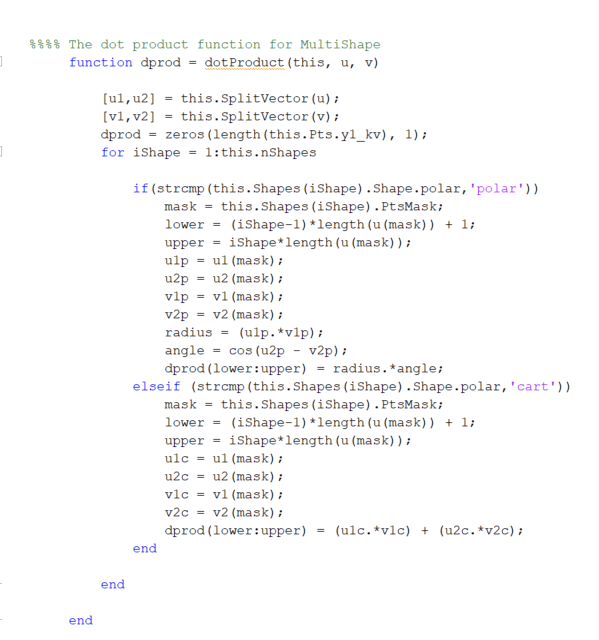
\includegraphics[scale=0.9]{dotProduct.png}
		\caption{Implementation of the dot product} 
		\label{FCode1}
	\end{figure}
	\begin{figure}[h]
	\centering
	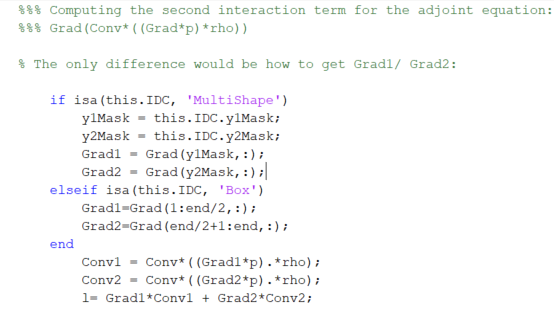
\includegraphics[scale=0.9]{adjoint.png}
	\caption{implementation of adjoint integral term} 
	\label{FCode2}
    \end{figure}
	The term we are trying to implement there is:
	\begin{align*}
	\nabla_r \int   V_2(|r-r'|)\nabla_{r'} p(r')dr'.
	\end{align*} 
	\section{Tests}
	Tested the forward problem and optimal control problem in different settings. It all seems to be working very well. 
	Forward Tests (Figure \ref{F0a}):
	\begin{itemize}
		\item Test 1: Compare computations on a box, with ADInf solution.
		\item Test 2: Compare on a box with AD Flow Neumann Exact solution.
		\item Test 3: Split box in MS code and compare to box in Box code using ADInf solution
		\item Test 3a: Same as 3 only checking that order of shapes don't matter.
		\item Test 4: Computing problem ADInf on wedge + quadrilateral
		\item Test 4a: Same as 4 only checking that order of shapes don't matter.
		\item ToyProblem 1: Computes no flux problem on two wedges and two quadrilaterals with constant 1 flow.
	\end{itemize} 
	Optimization Tests (Figure \ref{F0b}):
	\begin{itemize}
		\item Test 5: Comparing MS and Box code on a box with Neumann Flow Exact Problem
		\item Test 6: Split MS box in two parts and compare to box in Box code (same Exact solution)
		\item Test 7: Comparing on the box an interacting problem (problem one from paper)
		\item Test 8: Splitting MS box and comparing to Box code for interacting problem
	\end{itemize}
	\begin{figure}[h]
		\centering
		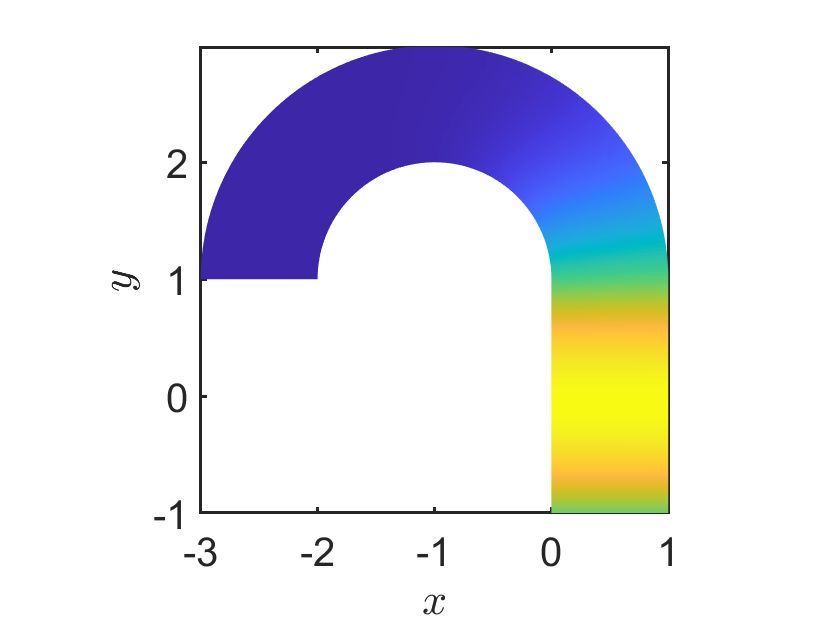
\includegraphics[scale=1]{T1.png}
		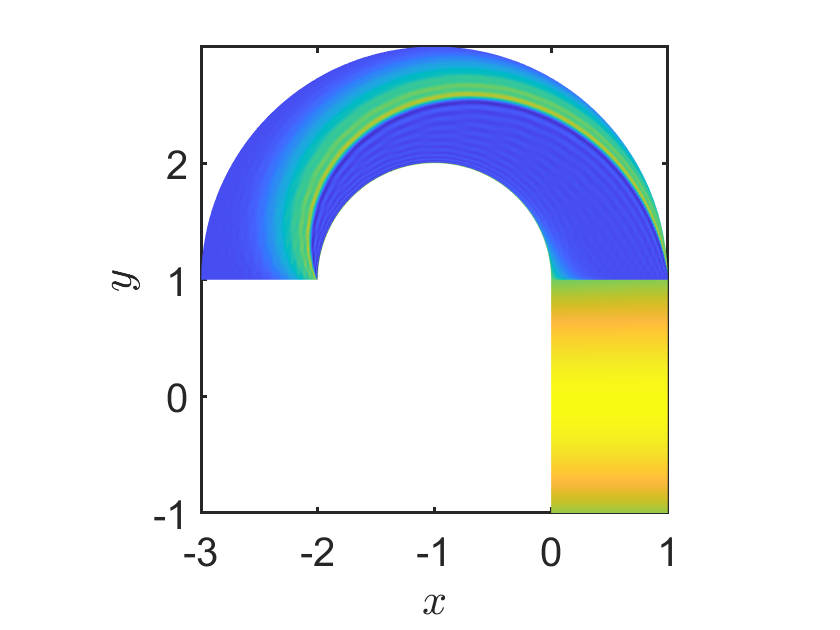
\includegraphics[scale=1]{T2.png}
		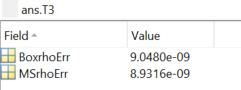
\includegraphics[scale=1]{T3.png}\\
		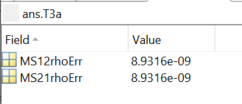
\includegraphics[scale=1]{T3a.png}
		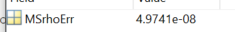
\includegraphics[scale=1]{T4.png}
		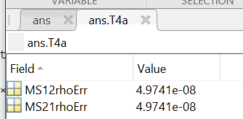
\includegraphics[scale=1]{T4a.png}
		\caption{Forward Test Solutions} 
		\label{F0a}
    \end{figure}
	\begin{figure}[h]
		\centering
		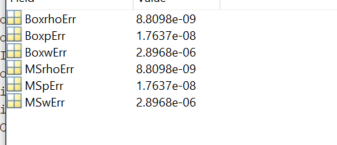
\includegraphics[scale=1]{T5.png}
		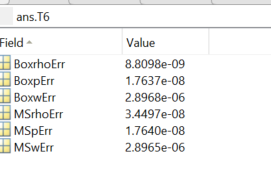
\includegraphics[scale=1]{T6.png}\\
		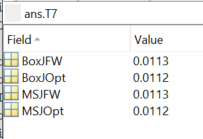
\includegraphics[scale=1]{T7.png}
		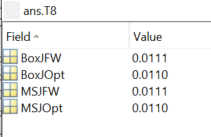
\includegraphics[scale=1]{T8.png}
		\caption{Optimization Test Solutions} 
		\label{F0b}
	\end{figure}
	
	\section*{Comparing Matching Conditions in Forward problem}
	Compared with ADinf exact solution. Matching two boxes (vs full box) in Figure \ref{F1} and matching two wedges (vs full wedge) in Figure \ref{F2}. Both show that the results are the same regardless of the matching method.
	\begin{figure}[h]
		\centering
		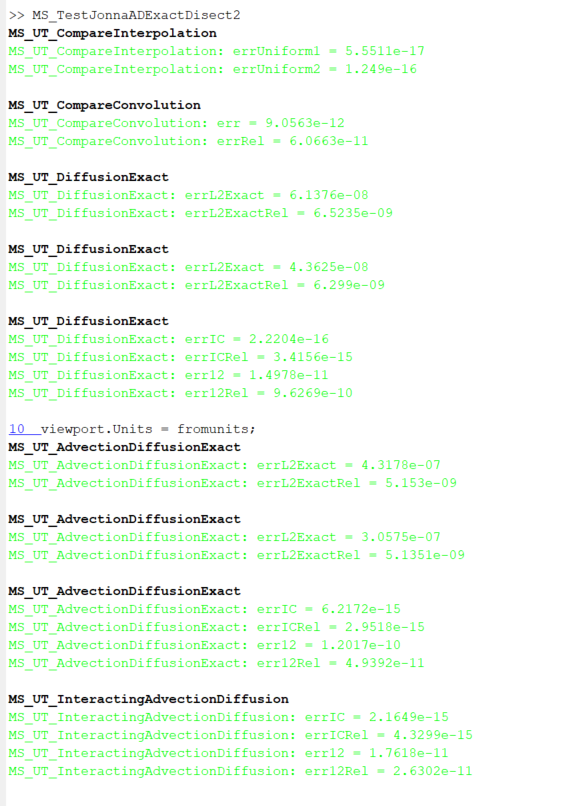
\includegraphics[scale=0.7]{rhoDymatch.png}
		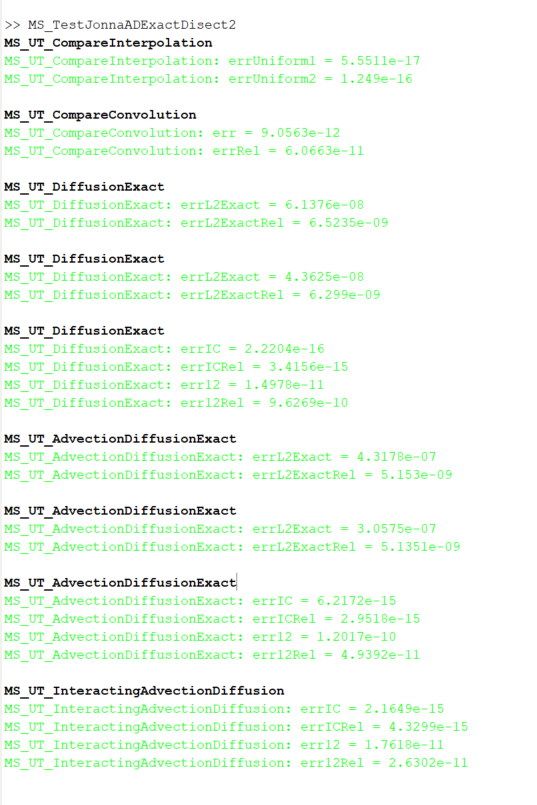
\includegraphics[scale=0.7]{rhoFluxmatch.png}
		\caption{Boxes with matching first derivative and flux} 
		\label{F1}
	\end{figure}
	\begin{figure}[h]
		\centering
		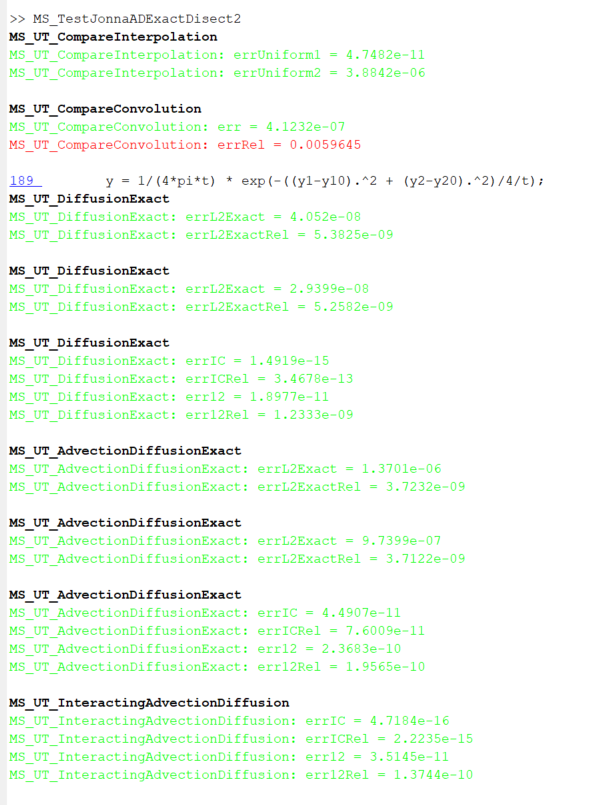
\includegraphics[scale=0.7]{rhoDyWedge.png}
		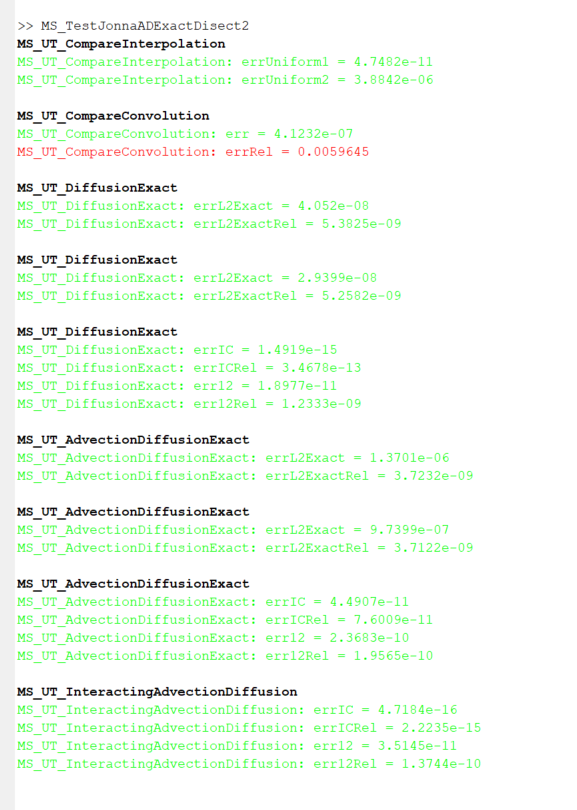
\includegraphics[scale=0.7]{rhoFluxWedge.png}
		\caption{Wedge with matching first derivative and flux} 
		\label{F2}
	\end{figure}
	\begin{figure}[h]
		\centering
		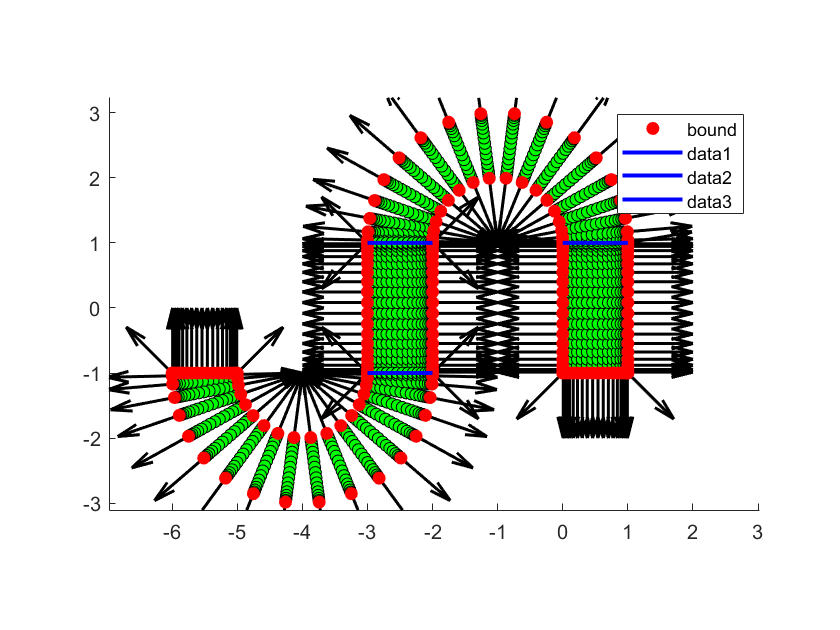
\includegraphics[scale=0.5]{dom1.png}
		\caption{Domain} 
		\label{FD1}
	\end{figure}
	Using the example with no flux and two wedges and two boxes (see Figure \ref{FD1}), the two matching methods are compared. The error in $\rho$ is $1.4292\times 10^{-10}$.
	
	
	\section{Finding distances between points that leave the domain}
	There must be a better way of doing this, because this seems impossibly inefficient, but the way I think of this is the following, see Figure \ref{FI}.
	For each pair of points $\vec x_1$, $\vec x_2$ do:
	\begin{enumerate}
		\item Check if points lie ON the boundary at first. 
		\item Find the linear function connecting $\vec x_1$, $\vec x_2$, $f$.
		\item Consider each boundary in the domain $[x_1, x_2]\times [y_1, y_2]$, in particular, each side of each boundary.
		\item If boundary is Cartesian:\\
		Choose two points $\vec b_1$, $\vec b_2$ on the boundary segment. Define the linear function connecting these two points, $h$. 
		\item Find the intersection between $f$ and $h$, in particular check $m_1 - m_2 \neq 0 $. Check that the solution $(a,b) \in  [x_1, x_2]\times [y_1, y_2]$.
		\item If boundary is Polar:\\
		Either convert to Cartesian or get $f$ in polar.
	\end{enumerate}
		\begin{figure}[h]
		\centering
		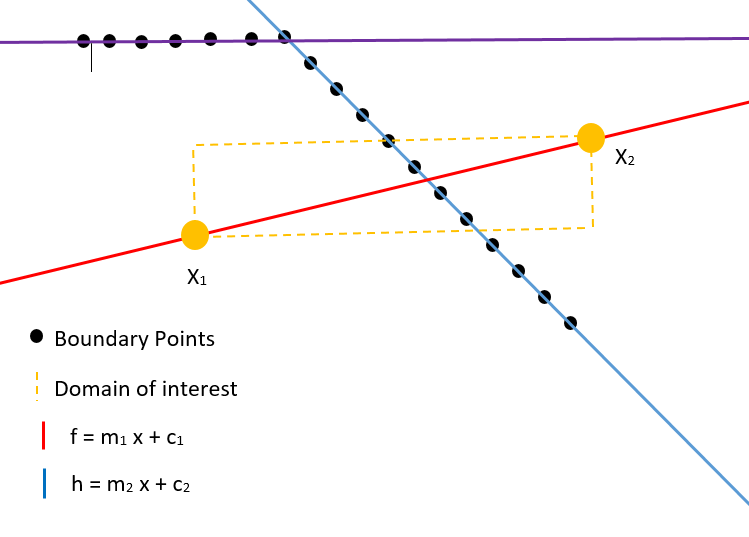
\includegraphics[scale=0.7]{Intersection.png}
		\caption{Intersection} 
		\label{FI}
    	\end{figure}
    
    
    
    \section{OCP on MultiShape}
    
    \subsection{Example 1}
    We choose the initial condition for $\rho$ to be $exp(-2((y1 - 0.5 )^2 + (y2 + 0.5)^2))$ and solve a forward problem with constant velocity of strength one, see Figure \ref{FTest1FW}.
    \begin{figure}[h]
    	\centering
    	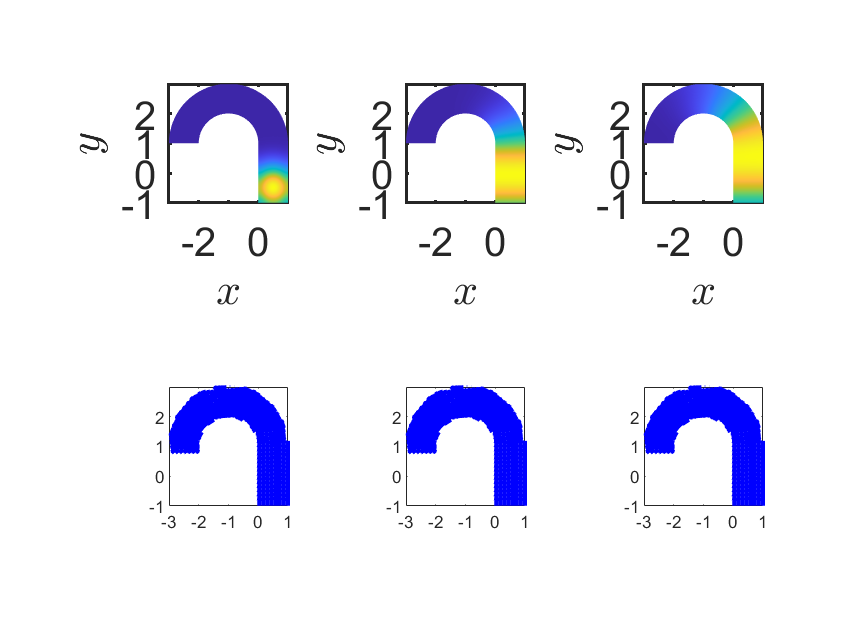
\includegraphics[scale=0.7]{Test10FW.png}
    	\caption{Test1 Forward $t =1, 10, 19, n = 20$} 
    	\label{FTest1FW}
    \end{figure}
    Then we use this forward solution as a target in the OCP, with initial velocity zero. We set $\beta = 10^{-3}$, we solve with tolerances $10^{-7}/ 10^{-3}$, because of time constraints, and $n = 20$, $N = 20$. The solution can be seen in Figure \ref{FTest1Opt}. As expected, the control follows the particle mass. It takes $452$ iterations, but the time it takes is $2 \times 10^4$. We get $J_{FW} = 0.0206$, $J_{Opt} = 0.0020$. 
    \begin{figure}[h]
    	\centering
    	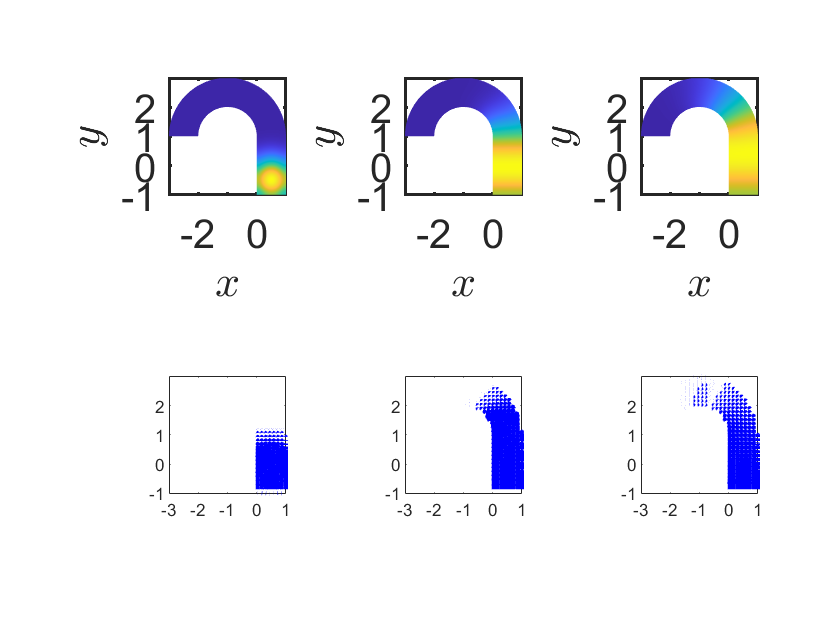
\includegraphics[scale=0.7]{Test10Opt.png}
    	\caption{Test1 Optimization $t =1, 10, 19, n = 20$} 
    	\label{FTest1Opt}
    \end{figure}
    We then choose $\kappa = -1$ and get $J_{FW} = 0.0251$, $J_{Opt} = 0.0020$, in $454$ iterations taking $ 1\times 10^4$ in time. We can see the results in Figures \ref{FTest1n1FW} and \ref{FTest1n1Opt}.
    \begin{figure}[h]
    	\centering
    	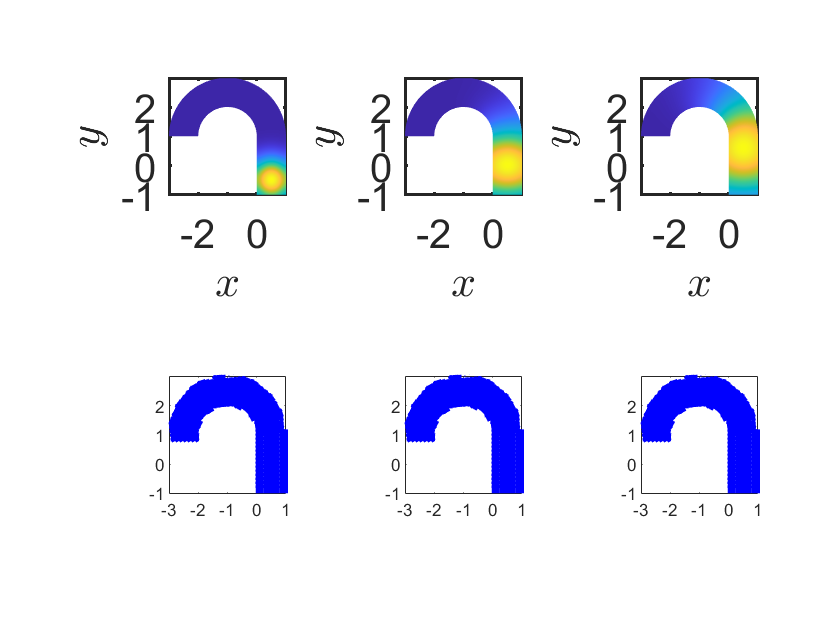
\includegraphics[scale=0.7]{Test10n1FW.png}
    	\caption{Test1 Forward $\kappa = -1$, $t =1, 10, 19, n = 20$} 
    	\label{FTest1n1FW}
    \end{figure}
    \begin{figure}[h]
    	\centering
    	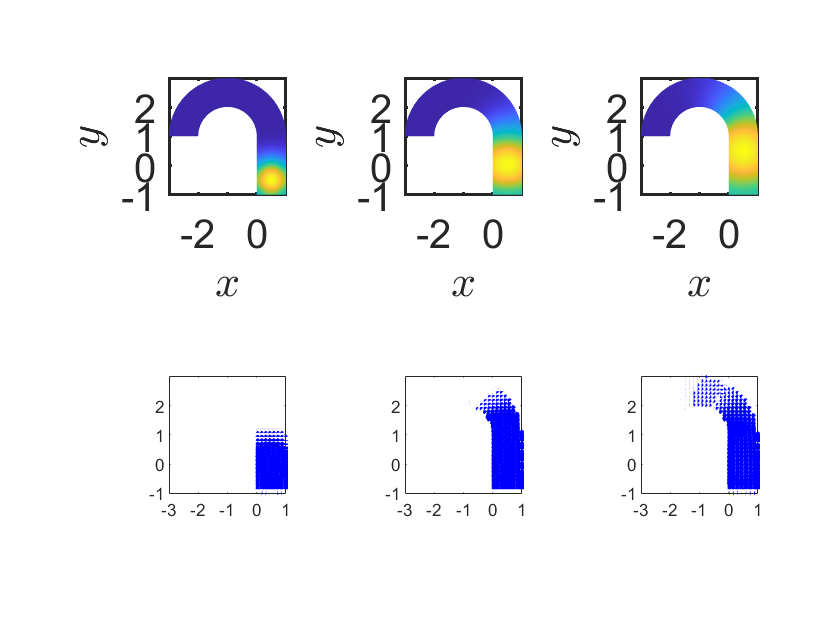
\includegraphics[scale=0.7]{Test10n1Opt.png}
    	\caption{Test1 Optimization $\kappa = -1$, $t =1, 10, 19, n = 20$} 
    	\label{FTest1n1Opt}
    \end{figure}
    We can do the same for $\kappa = 1$. We get $J_{FW} = 0.0176$, $J_{Opt} = 0.0020$, in $451$ iterations taking $ 1\times 10^4$ in time. We can see the results in Figures \ref{FTest11FW} and \ref{FTest11Opt}.
    \begin{figure}[h]
    	\centering
    	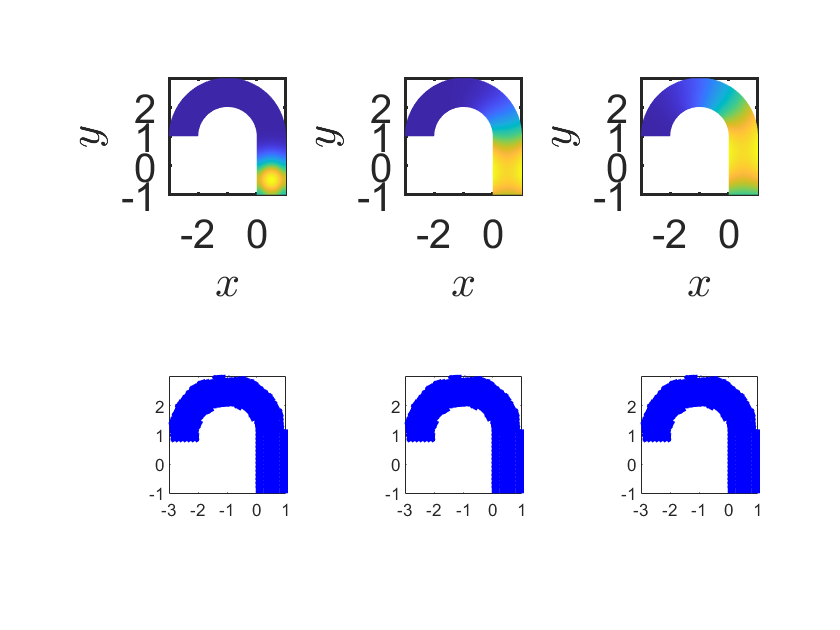
\includegraphics[scale=0.7]{Test101FW.png}
    	\caption{Test1 Forward $\kappa = 1$, $t =1, 10, 19, n = 20$} 
    	\label{FTest11FW}
    \end{figure}
    \begin{figure}[h]
    	\centering
    	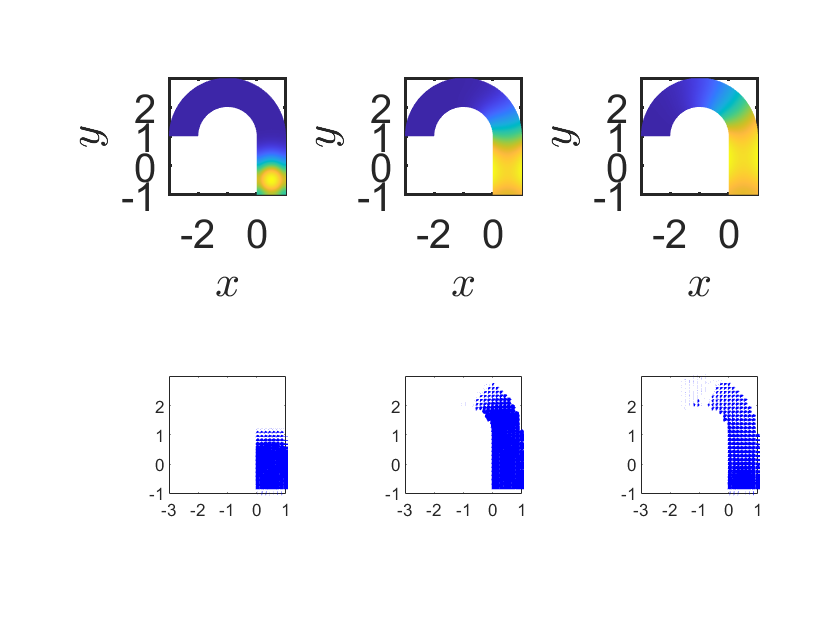
\includegraphics[scale=0.7]{Test101Opt.png}
    	\caption{Test1 Optimization $\kappa = 1$ $t =1, 10, 19, n = 20$} 
    	\label{FTest11Opt}
    \end{figure}
    
    \subsection{Example 2}
    We choose the initial condition for $\rho$ to be $exp(-2((y1 - 0.5 )^2 + (y2 + 0.5)^2))$ and solve a forward problem with constant velocity of strength five, see Figure \ref{FTest2FW}.
    \begin{figure}[h]
    	\centering
    	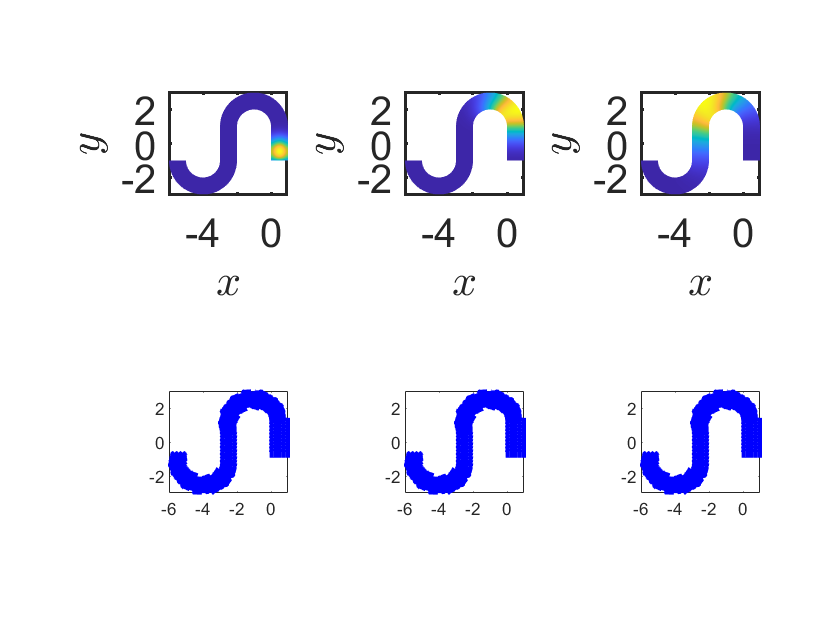
\includegraphics[scale=0.7]{Test11FW.png}
    	\caption{Test2 Forward $t =1, 10, 19, n = 20$} 
    	\label{FTest2FW}
    \end{figure}
    Then we use this forward solution as a target in the OCP, with initial velocity zero. We set $\beta = 10^{-3}$, we solve with tolerances $10^{-7}/ 10^{-3}$, because of time constraints, and $n = 20$, $N = 20$. The solution can be seen in Figure \ref{FTest2Opt}. Again, as expected, the control follows the particle mass. It takes $ 587$ iterations, but the time it takes is $ 5 \times 10^4$. We get $J_{FW} =  0.1921$, $J_{Opt} =  0.0326$. 
    \begin{figure}[h]
    	\centering
    	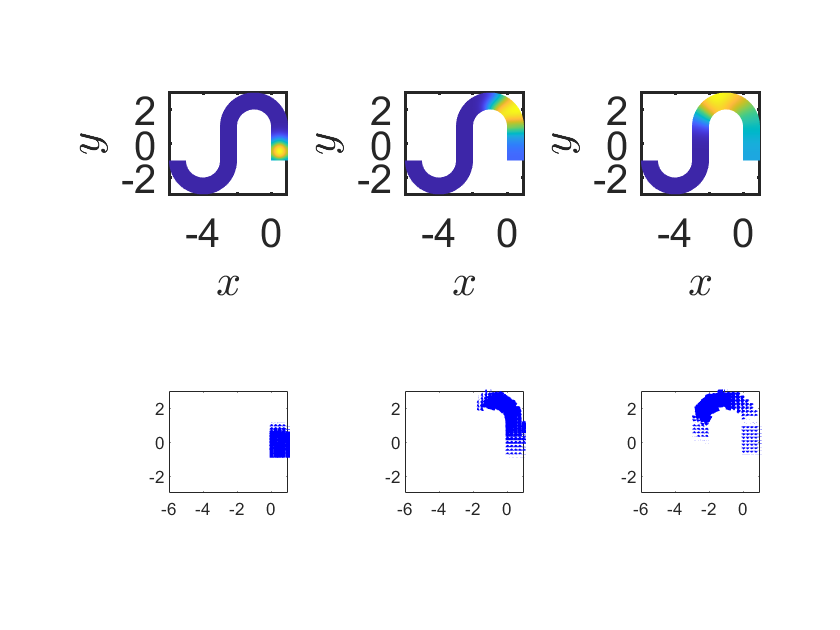
\includegraphics[scale=0.7]{Test11Opt.png}
    	\caption{Test2 Optimization $t =1, 10, 19, n = 20$} 
    	\label{FTest2Opt}
    \end{figure}
    
    \section{Things that do not work}
    Giving the forward problem with the constant velocity as initial guess AND as target for the OCP and ask it to do better. It immediately diverges. Maybe too advection dominant?\\
    Considering problem 2 above with velocity strength 10 and interaction term. Diverges. Advection dominance?\\
    In and outflow BCs. Diverges immediately. Correct implementation? Or maybe this restricts too much and we can't actually change the flow much...  
    
    
    
    
\end{document}